\documentclass[12pt]{article}

\usepackage{mathtools} 
\usepackage{cite}
\usepackage{graphicx}
\usepackage{listings}
\usepackage{wrapfig}

\title{The hunt for the next generation battery}

\begin{document}
\maketitle
\begin{abstract}
High density non-rechargeable energy batteries barely store one twentieth the energy of liquid hydrocarbons. Characterizing the mechanics of reactions to build a simulation that is capable of determining if a reaction is a battery, a rechargeable one, and the potential performance characteristics is complex. Training simulation predictors to reduce the complexity at certain steps augmented with real data can help to ensure that potential candidate reactions for analysis are of high quality.
\end{abstract}
\section{Generating Reactions}
Consider a system that constructs reactions from a given set of compounds. In the general case there are $2^{Reactants} * 2^{Products}$ potential reactions to consider. Using a matrix reduction technique \{cite here\} that balances coefficients and determines if the compound is a product or reactant only the set $2^{Compounds}$ needs to be considered. Reactions can be linear combinations of multiple other unique or linear reactions so the space can be divided into $\{LinearCombination,UniqueReaction,NotAReaction\}$. Enumerating only the $\{UniqueReaction\}$ set is thus the first goal of complexity reduction. All reactions generated by such a system must be checked and verified to be mass, oxidation, charge, spin, etc balanced. To represent enumeration of this space a forest of trees representation is constructed where each node is a compound and the path from the tree-root to the node is the set of compounds under consideration.
\newpage
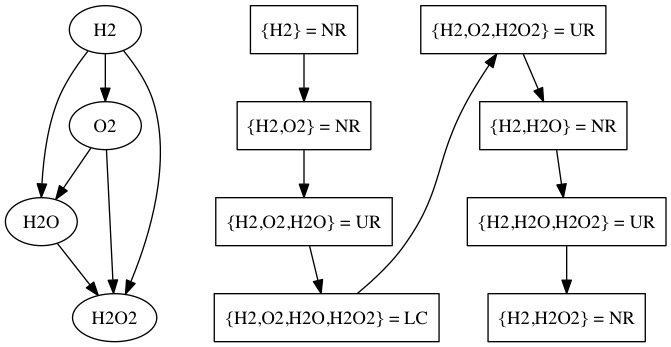
\includegraphics[scale=.50]{tree_set}

$NR$ = Not a Reaction, $UR$ = Unique Reaction, $LC$ = Linear Combination

The resulting set of unique reactions for a given set of compounds is a hypergraph of all potential mass law obeying reactions.  Each node is a compound, each edge is a reaction with mass balanced coefficients as connection weights. Negative and positive weights represent sides of the equation.\\
 
 \begin{wrapfigure}{r}{0.5\textwidth}
  \begin{center}
    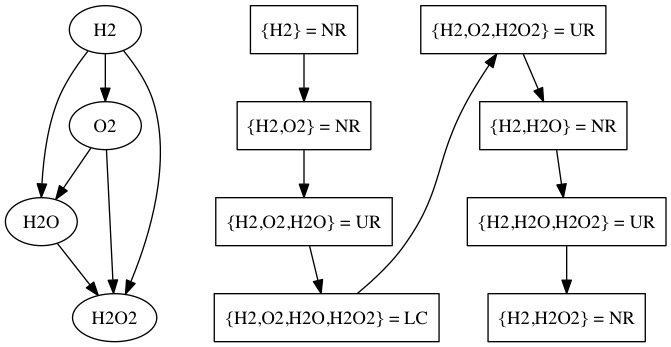
\includegraphics[width=0.48\textwidth]{reaction_hypergraph}
  \end{center}
\end{wrapfigure}

The result  is a complete reaction hypergraph network which then be explored. Each reaction edge is guaranteed to be unique and represent a specific potential reaction. These reactions are not characterized, they represent valid mass balanced potential reactions. Some sub-spaces $\leq 2^{1000}$ can and have been computed quickly. Heuristics can sidestep complexity and size but the upper bound grows exponentially. The next step of filtering out reactions to only those which comply with oxidation - reduction mechanics will reduce the reactions to consider. The remaining reactions shall be analyzed with consideration and respect to $\{H_2,O_2,H_2O,H^+,HO^-\}$ which will probably act as charge carriers in the system.
\end{document}